\begin{maintask}{3-1}
  \subsection*{課題内容}
  PythonのDNSリゾルバ(dnspython)で，IPv4のみ対応のホストとIPv4/IPv6両対応のホストのA・AAAAレコードを引き，その通信を分析した．

  \subsection*{実験方法}
  \begin{enumerate}
    \item ひな型を自分のホームにコピー
      \begin{minted}{zsh}
        cd; cp -r /shares/dns .; chmod -R u+w dns; cd dns
      \end{minted}

    \item ホスト名ごとに，キャプチャ開始，q\_hostnameの書き換え，実行，キャプチャ停止を行う
      \begin{minted}{zsh}
        (IPv4のみ)  tcpdump -i eth1 -s 0 -w day3_1_v4.pcap 'not port 4200'    (1つ目のターミナル)
                    sed -i "s/^q_hostname=.*/q_hostname='www.city.sapporo.jp'/" dnspython_sample.py
                    ./dnspython_sample.py
        (両対応)    tcpdump -i eth1 -s 0 -w day3_1_v46.pcap 'not port 4200'   (1つ目のターミナル)
                    sed -i "s/^q_hostname=.*/q_hostname='www.pref.hokkaido.lg.jp'/" dnspython_sample.py
                    ./dnspython_sample.py
      \end{minted}

    \item 各pcapをWiresharkで開き，次のフィルタを適用
      \begin{minted}{text}
        udp.port == 53 && !(dns.qry.type == 12)
      \end{minted}
      逆引き(PTR, Type 12)は本課題と無関係なので除外した．
  \end{enumerate}

  \subsection*{結果}
  tcpdumpの実行結果と，dnspython\_sample.pyの実行結果を
  出力\ref{out:tcpdump_31_v4}，
  出力\ref{out:tcpdump_31_v46}，
  出力\ref{out:dnspy_v4}，
  出力\ref{out:dnspy_v46}
  に示した．

  \begin{termout}[H]
    \caption{tcpdump(IPv4のみのホスト) の実行結果}\label{out:tcpdump_31_v4}
    \begin{minted}{zsh}
    guest@host82:~/dns$ tcpdump -i eth1 -s 0 -w day3_1_v4.pcap 'not port 4200'
    tcpdump: listening on eth1, link-type EN10MB (Ethernet), capture size 262144 bytes
    ^C58 packets captured
    60 packets received by filter
    0 packets dropped by kernel
    \end{minted}
  \end{termout}

  \begin{termout}[H]
    \caption{tcpdump(両対応のホスト) の実行結果}\label{out:tcpdump_31_v46}
    \begin{minted}{zsh}
    guest@host82:~/dns$ tcpdump -i eth1 -s 0 -w day3_1_v46.pcap 'not port 4200'
    tcpdump: listening on eth1, link-type EN10MB (Ethernet), capture size 262144 bytes
    ^C22 packets captured
    24 packets received by filter
    0 packets dropped by kernel
    \end{minted}
  \end{termout}

  \begin{termout}[H]
    \caption{dnspython\_sample.py(www.city.sapporo.jp) の実行結果}\label{out:dnspy_v4}
    \begin{minted}{zsh}
    guest@host82:~/dns$ ./dnspython_sample.py
    Querying hostname: www.city.sapporo.jp
    A records are:
      45.60.112.77
      Replied nameserver: 133.87.1.11 (53)
    AAAA records: No answer from the resolver.
    \end{minted}
  \end{termout}

  \begin{termout}[H]
    \caption{dnspython\_sample.py(www.pref.hokkaido.lg.jp) の実行結果}\label{out:dnspy_v46}
    \begin{minted}{zsh}
    guest@host82:~/dns$ ./dnspython_sample.py
    Querying hostname: www.pref.hokkaido.lg.jp
    A records are:
      45.60.112.77
      Replied nameserver: 133.87.1.11 (53)
    AAAA records are:
      2a02:e980:10e::4d
      Replied nameserver: 133.87.1.11 (53)
    \end{minted}
  \end{termout}

  \begin{figure}[h]
    \centering
    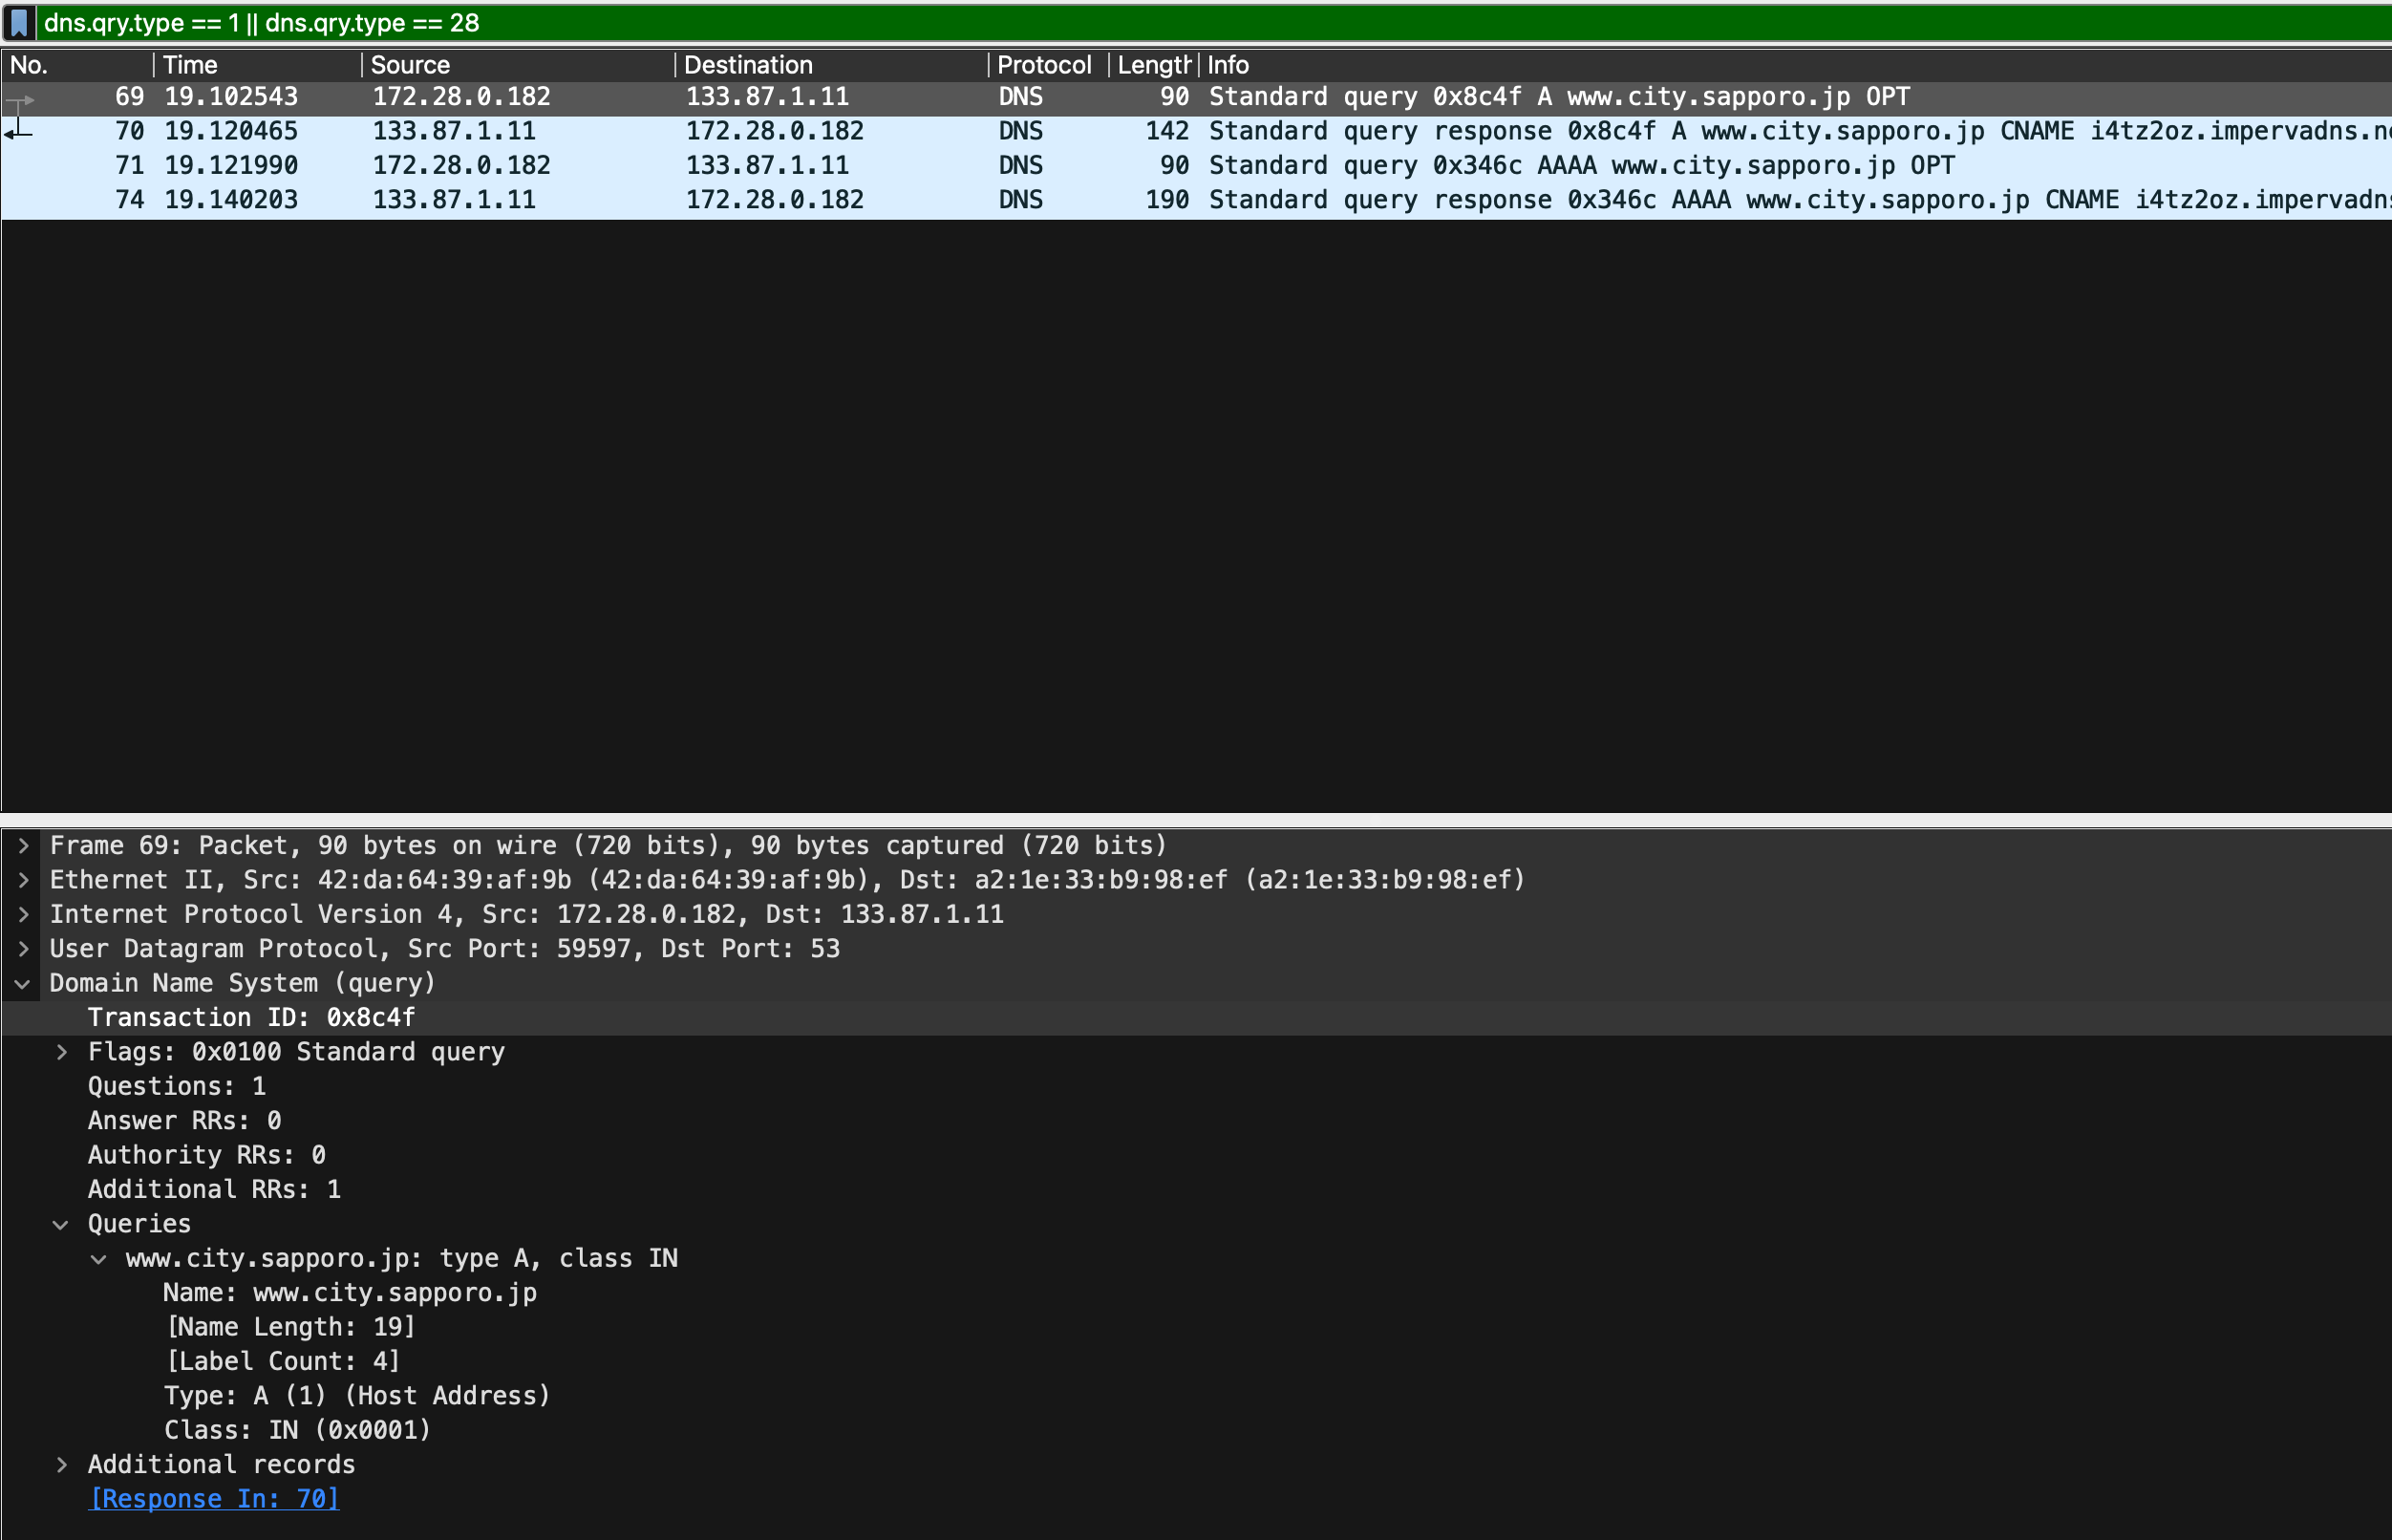
\includegraphics[width=0.98\columnwidth]{fig/wireshark_31_v4_query.png}
    \caption{IPv4のみのホストのA・AAAAの問い合わせ}
    \label{fig:ws_31_v4_query}
  \end{figure}

  \begin{figure}[h]
    \centering
    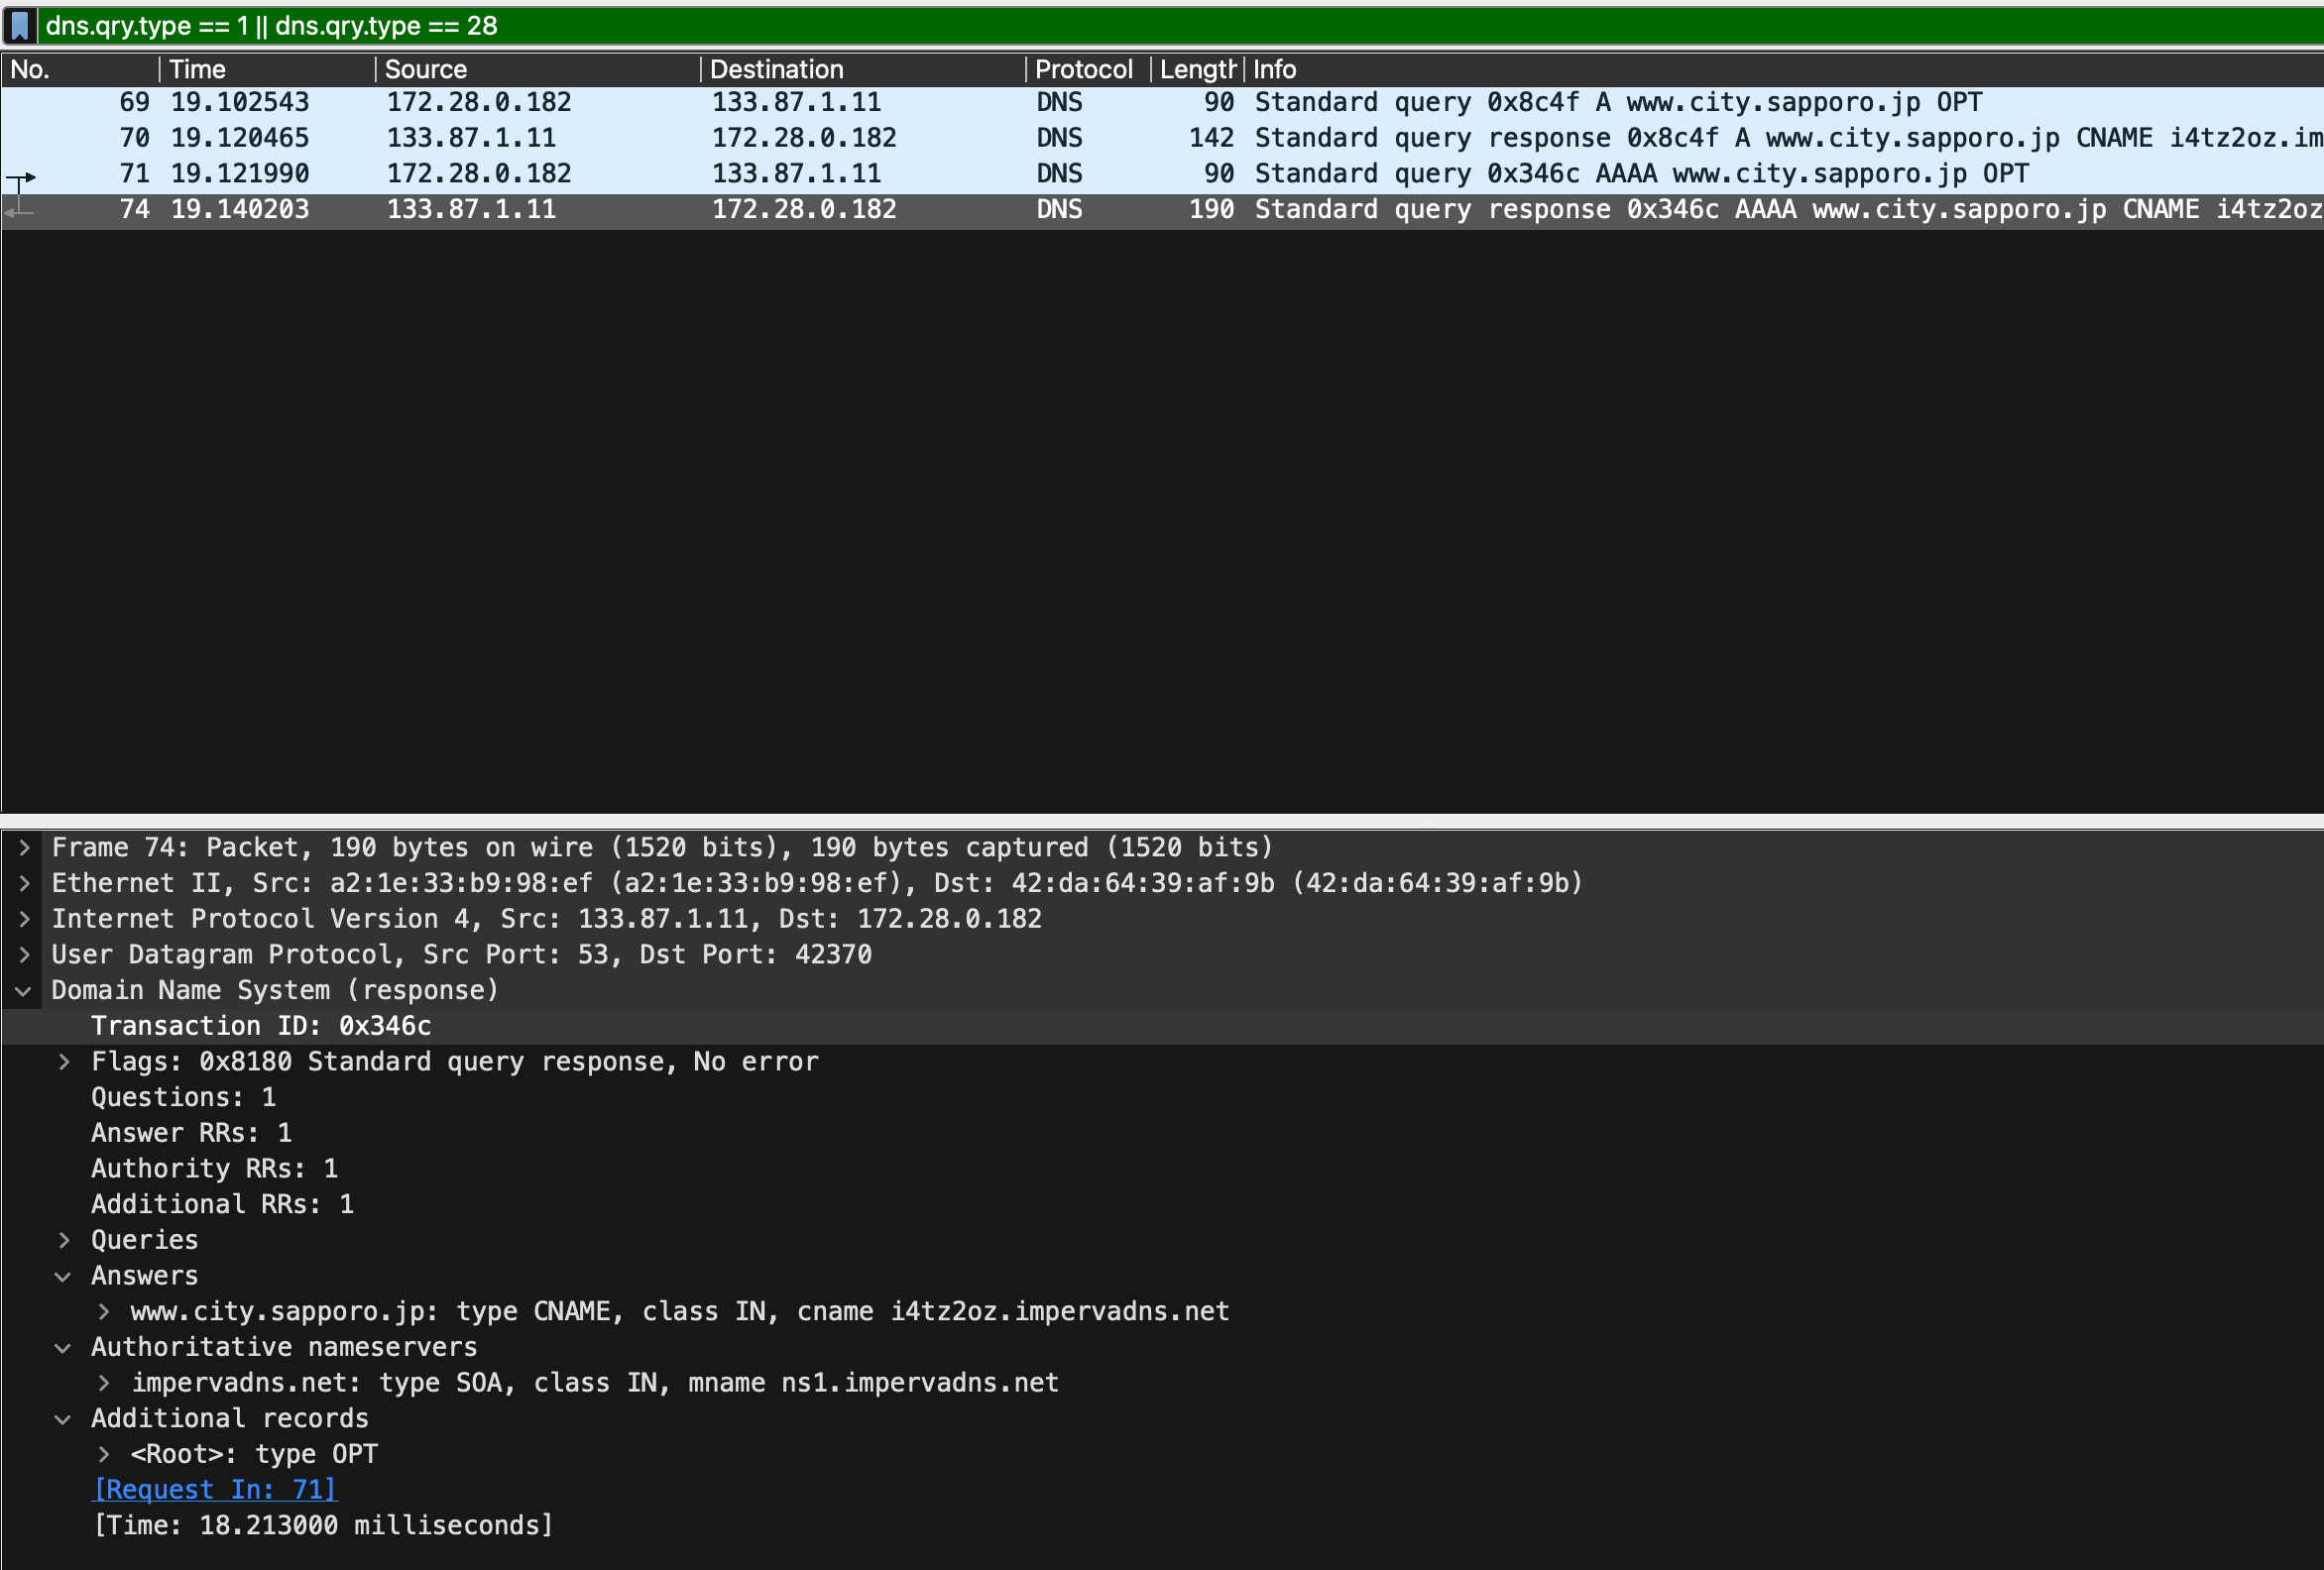
\includegraphics[width=0.98\columnwidth]{fig/wireshark_31_v4_answer.png}
    \caption{IPv4のみのホストのA・AAAAの応答}
    \label{fig:ws_31_v4_answer}
  \end{figure}

  \begin{figure}[h]
    \centering
    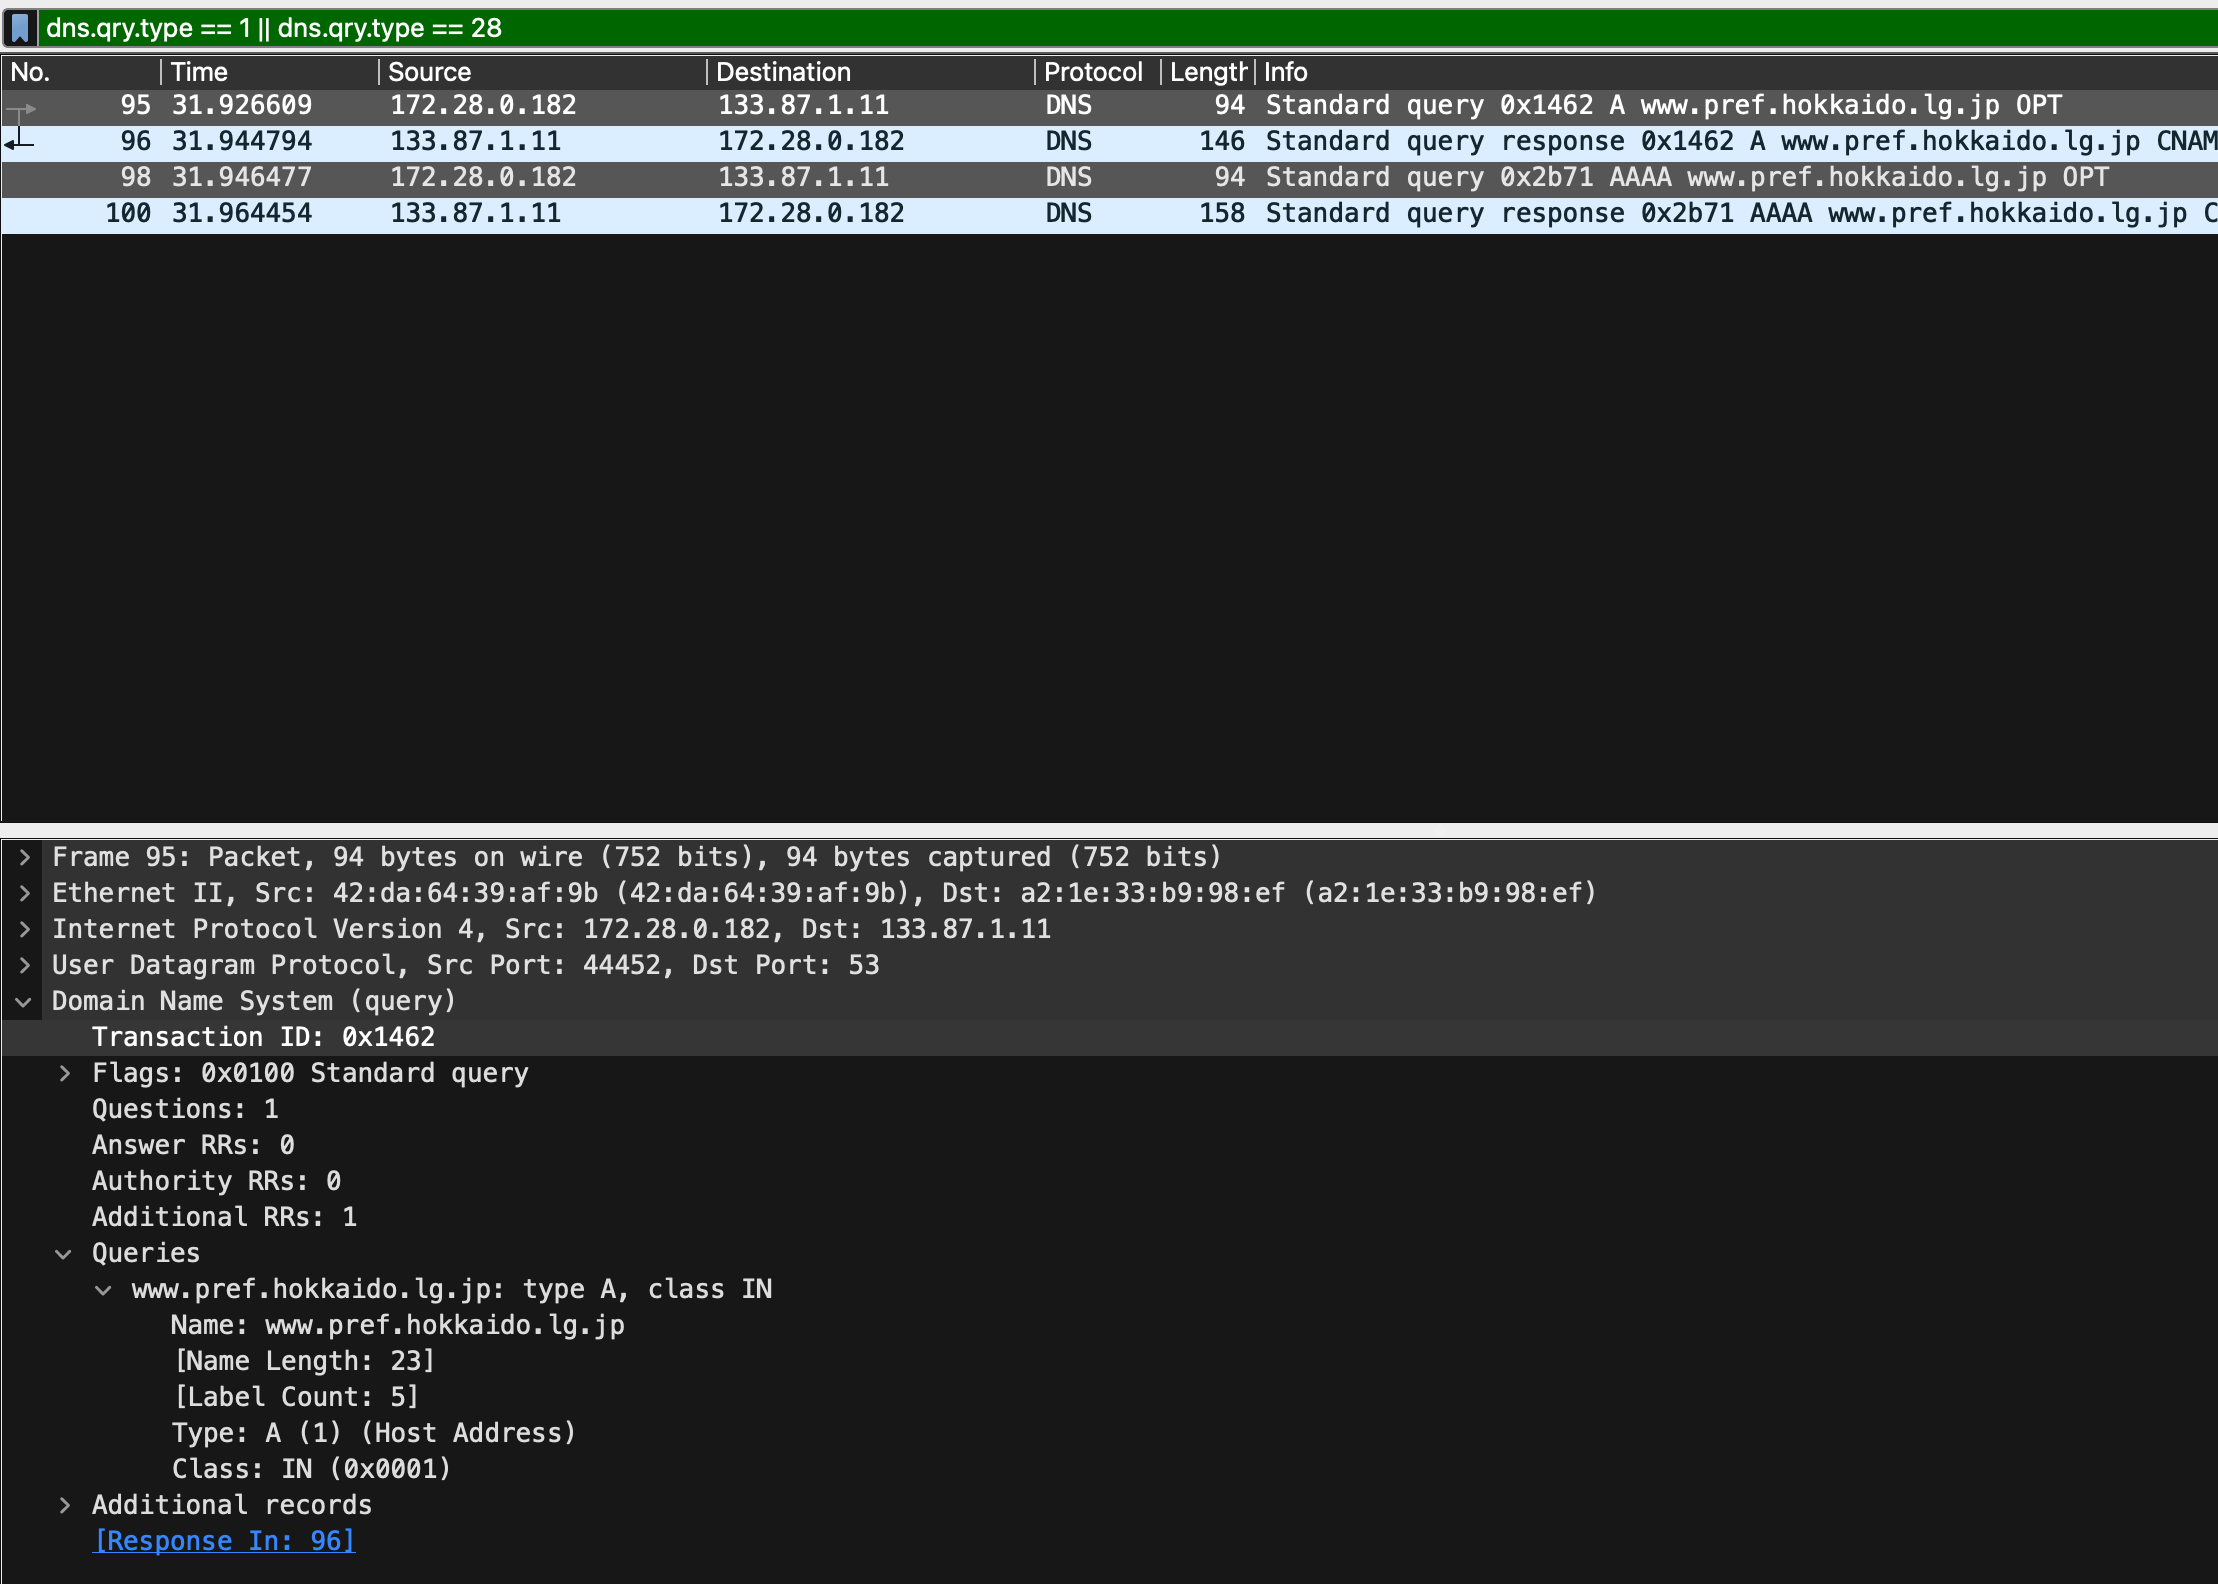
\includegraphics[width=0.98\columnwidth]{fig/wireshark_31_v46_query.png}
    \caption{両対応のホストのA・AAAAの問い合わせ}
    \label{fig:ws_31_v46_query}
  \end{figure}

  \begin{figure}[h]
    \centering
    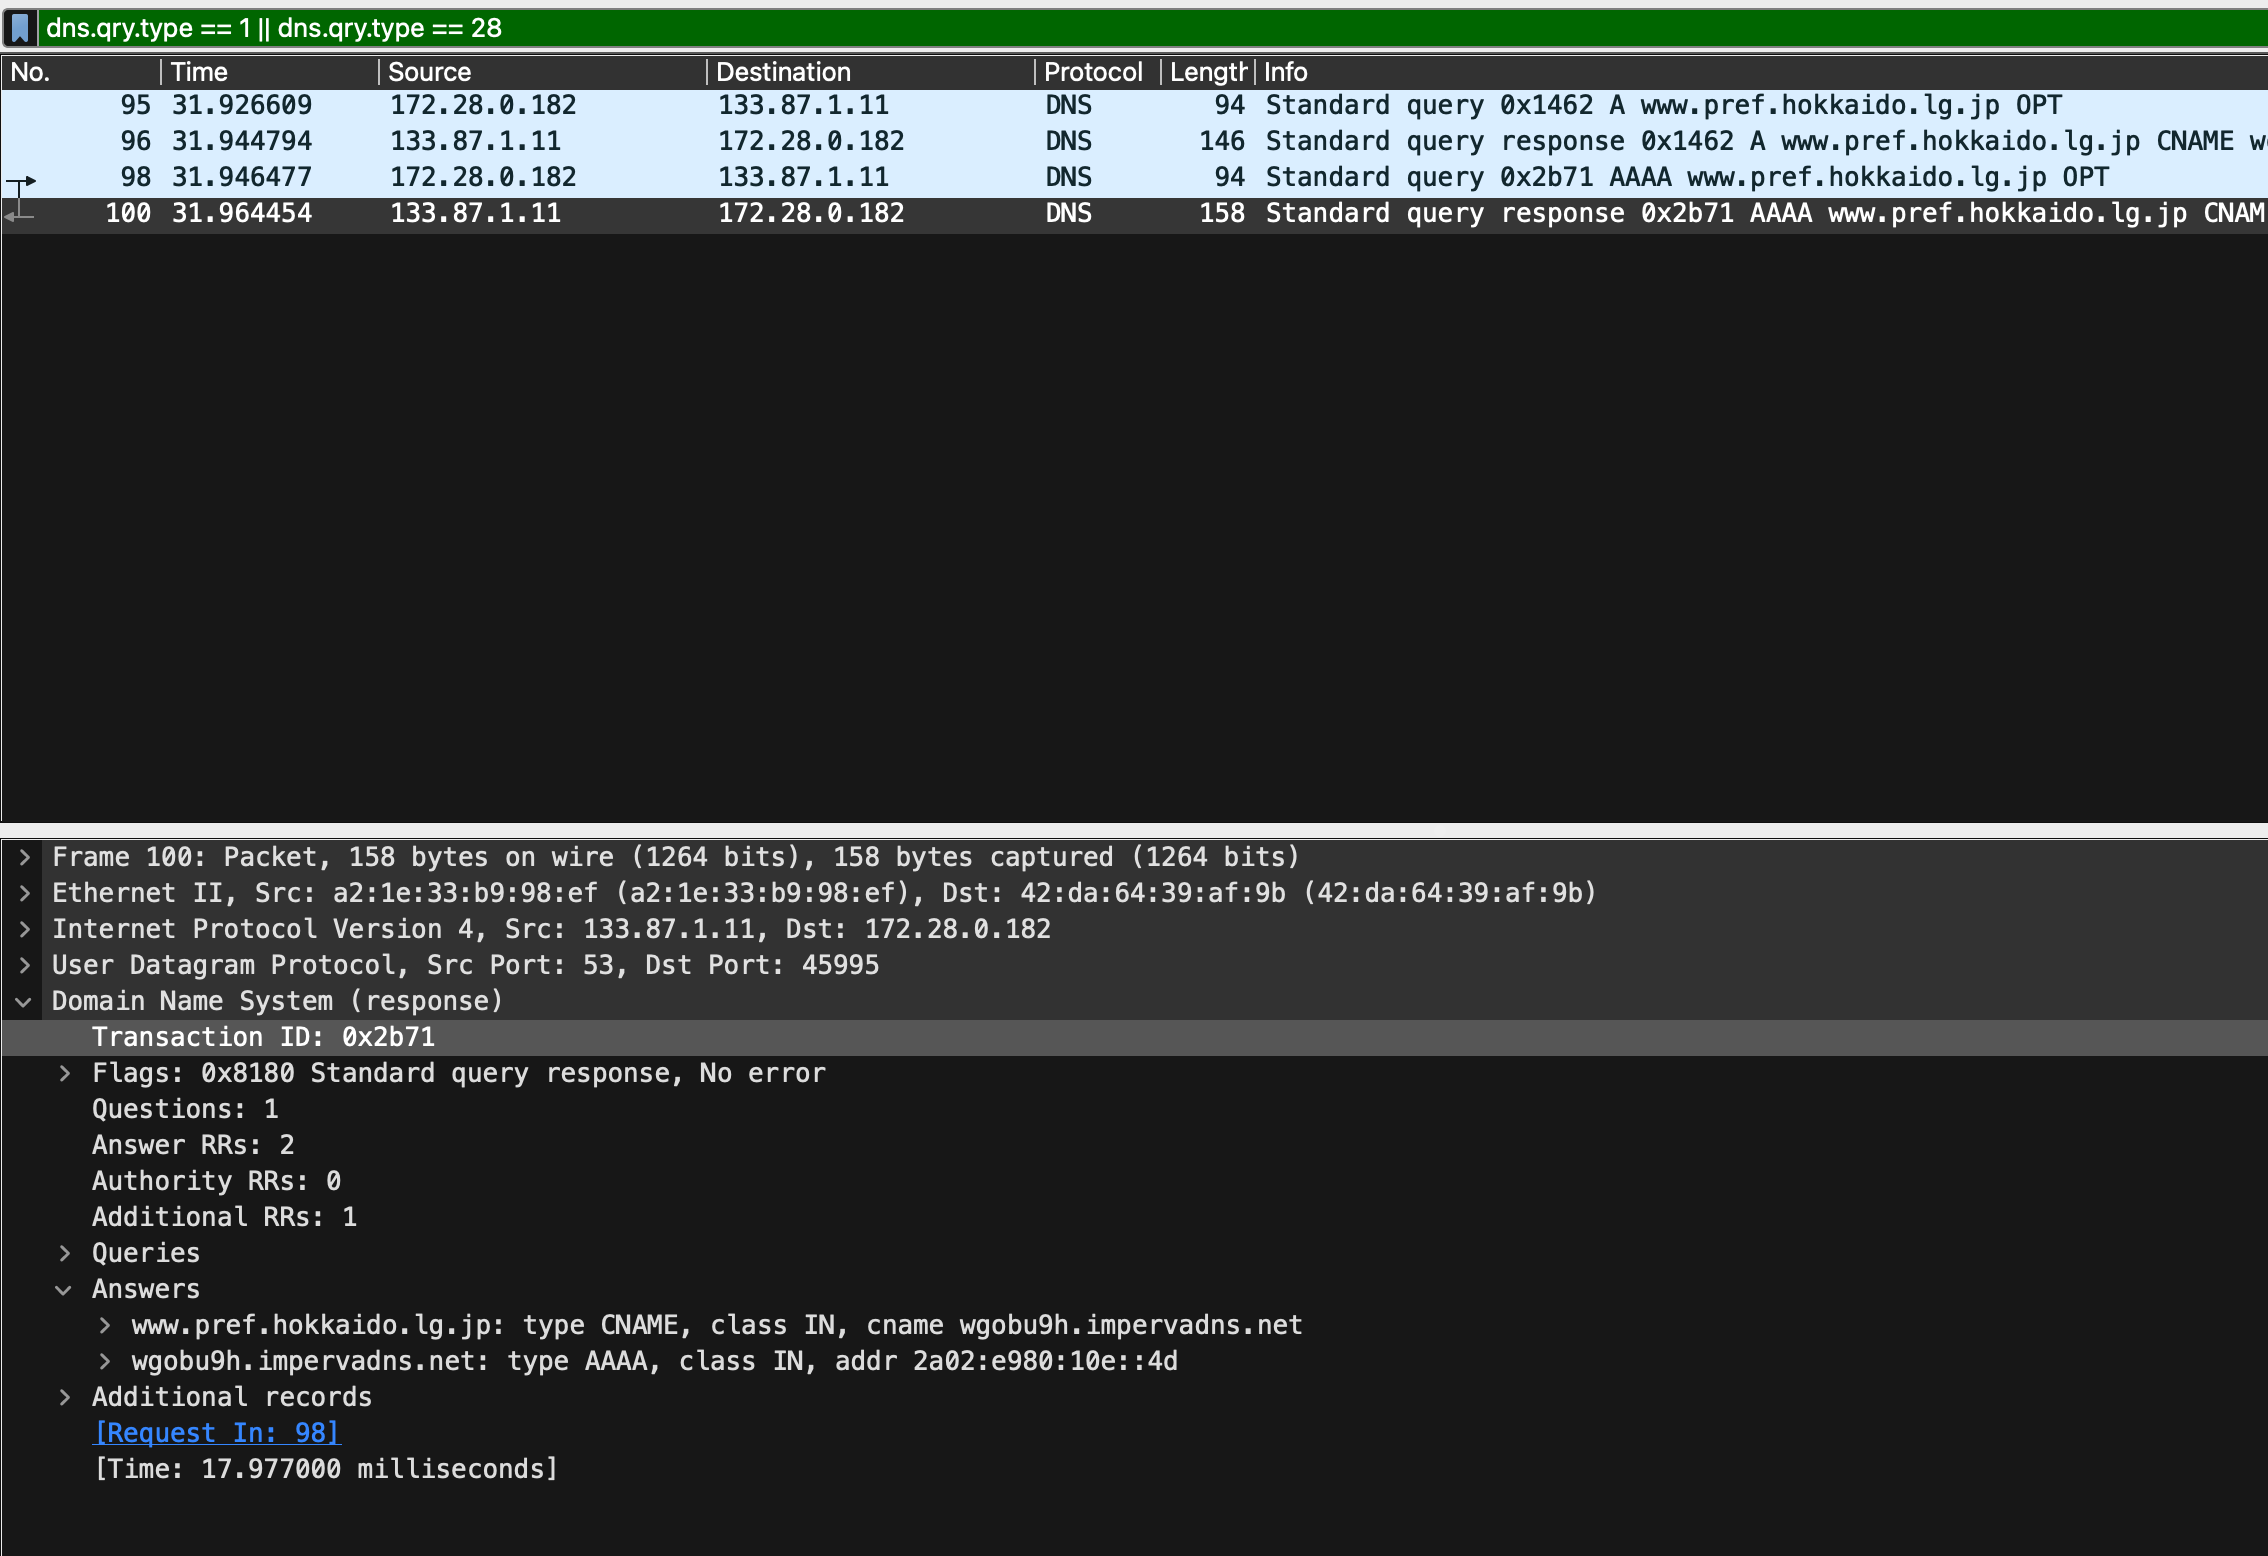
\includegraphics[width=0.98\columnwidth]{fig/wireshark_31_v46_answer.png}
    \caption{両対応のホストのA・AAAAの応答}
    \label{fig:ws_31_v46_answer}
  \end{figure}

  IPv4のみのホスト(www.city.sapporo.jp)では，図\ref{fig:ws_31_v4_query}のとおり，No.69でAレコード，No.71でAAAAレコードの問い合わせが，リゾルバ133.87.1.11(UDP 53番ポート)に送られた．図\ref{fig:ws_31_v4_answer}では，Aの応答(No.70)には，CNAME(i4tz2oz.impervadns.net)を経由してアドレス45.60.112.77(TTL 119秒)が含まれている一方，AAAAの応答(No.74)にはCNAMEとSOAのみが含まれ，AAAAレコードはなかった．これは，このホストがIPv6のアドレスを持たないことを示す．出力\ref{out:dnspy_v4}でも，Aレコードとして45.60.112.77が1件表示された一方，AAAAは``No answer from the resolver''と表示されており，パケットの内容と一致する．

  両対応のホスト(www.pref.hokkaido.lg.jp)では，図\ref{fig:ws_31_v46_query}のとおり，No.95でAレコード，No.98でAAAAレコードの問い合わせが同様にリゾルバ133.87.1.11に送られた．図\ref{fig:ws_31_v46_answer}では，Aの応答(No.96)にIPv4アドレス45.60.112.77(TTL 46秒)，AAAAの応答(No.100)にIPv6アドレス2a02:e980:10e::4d(TTL 46秒)が含まれた．どちらの応答にも，www.pref.hokkaido.lg.jpからwgobu9h.impervadns.netへのCNAMEが含まれ，その先のAレコード，AAAAレコードとしてアドレスが得られている．出力\ref{out:dnspy_v46}にも，同じ2つのアドレスが表示されている．

  2つのホストを比べると，どちらでもAとAAAAの2種類の問い合わせが同じリゾルバ(133.87.1.11)に送られており，問い合わせの手順は同じである．違いは応答の内容にあり，IPv4のみのホストではAAAAの応答にアドレスがなく，両対応のホストでは両方のアドレスが得られた．また，2つのホストのAレコードは，どちらも45.60.112.77と同じ値であった．これは，どちらのホストもimpervadns.net配下の名前へのCNAMEを経由しており(sapporoはi4tz2oz.impervadns.net，hokkaidoはwgobu9h.impervadns.net)，同じ事業者のサービス上に置かれているためと考えられる．また，AとAAAAの問い合わせは並行ではなく順に送られていた．Aの応答を受け取った約1.5ミリ秒後(No.70とNo.71の間)にAAAAの問い合わせが送られており，両対応のホストでも同様に，Aの応答(No.96)の約1.7ミリ秒後にAAAAの問い合わせ(No.98)が送られている．
\end{maintask}
